\documentclass[11pt]{article}

% --- Page layout ---
\usepackage[a4paper,margin=2cm]{geometry}   % A4 paper with 2cm margins
\usepackage{multicol}                       % Support for multiple columns
\setlength{\columnsep}{1cm}                % Space between columns
\setlength{\columnseprule}{0.4pt}          % Vertical line between columns

% --- Typography and section formatting ---
\usepackage{titlesec}                       % Custom section title formatting
\titleformat{\section}{\normalfont\Large\bfseries}{}{0pt}{} % Section format
\titleformat{\subsection}{\normalfont\large\bfseries}{}{0pt}{} % Subsection format
\usepackage{parskip}                        % Adds space between paragraphs, no indent

% --- Lists and boxes ---
\usepackage{enumitem}                       % Customise list spacing and bullets
\usepackage[most]{tcolorbox}               % Boxes for Executive Summary
\tcbset{
	colback=blue!5,       % Light blue background
	colframe=black,       % Border color
	boxrule=0.5pt,        % Border thickness
	arc=1mm,              % Rounded corners
	left=6pt, right=6pt, top=6pt, bottom=6pt  % Padding
}

% --- Figures and tables ---
\usepackage{graphicx}                       % Insert images
\usepackage{float}                          % [H] float positioning
\usepackage{booktabs}                       % Nicer tables
\usepackage{caption}                        % Custom caption formatting
\captionsetup[figure]{justification=centering} % Center figure captions

% --- END of preamble ---

\begin{document}
	
	\begin{center}
		\LARGE\textbf{Policy Brief: Does High Homeownership Raise Youth Unemployment in Europe?}
	\end{center}
	
	\begin{multicols}{2}
		
		\section*{Executive Summary}
		
		\vspace{-1em}
		
		\begin{tcolorbox}
			\begin{itemize}[left=0.3em, labelsep=0.5em, labelwidth=0.6em, itemsep=0pt, topsep=0pt]
				\item In 2011, youth unemployment and homeownership showed a \textbf{moderate, statistically significant positive correlation} (\textit{r = 0.57, p < 0.01}).
				\item By 2018, the relationship had \textbf{weakened} and was \textbf{not statistically significant} (\textit{r = 0.16, p = 0.41}), likely reflecting post-crisis labour market recovery.
				\item Fixed-effects models show that \textbf{lagged homeownership} is linked to a \textbf{modest but significant} rise in youth unemployment (\textit{$\beta$ = 0.023}), even after controlling for year and country differences.
				\item \textbf{Demographic controls}, including age structure and education, were excluded due to \textbf{statistical insignificance} and \textbf{minimal contribution} to model fit.
				\item The relationship is strongest in countries with \textbf{rigid housing markets}  \textbf{(Greece, Spain, Italy)}, while \textbf{Malta, Norway} and \textbf{Slovenia} remain notable outliers.
			\end{itemize}
		\end{tcolorbox}

		\section*{Background and Context}
		In recent decades, governments across Europe have promoted homeownership as a pathway to wealth accumulation, stable communities, and civic participation. However, a growing body of research highlights potential labour market downsides to this approach. Blanchflower and Oswald (2013) argue that high ownership can increase unemployment by \textit{reducing geographic mobility}, \textit{lengthening commutes}, and \textit{discouraging new business formation}. These mechanisms may be especially relevant for young people (aged 16-24) who tend to rely more heavily on spatial mobility to access job opportunities.
				
		\vspace{-1em}
		
		\section*{Data and Methods}
		This analysis uses Eurostat data for 29 European countries (2011-2018), focusing on youth unemployment and homeownership rates. We examine their evolving relationship through scatterplots and Pearson's correlations. To address skewness, youth unemployment is log-transformed. Lagged homeownership serves as the key predictor to capture delayed labour market effects. Fixed-effects regressions control for year and country differences, isolating the impact of homeownership. Demographic controls were excluded due to statistical insignificance and limited contribution to model fit.
				
		\vspace{-1em}
		
		\section*{Key Findings}
		
		\subsection*{Descriptive Trends}
		
		\begin{figure}[H]
			\centering
			\caption{Homeownership vs. Youth Unemployment Across Europe (2011)}
			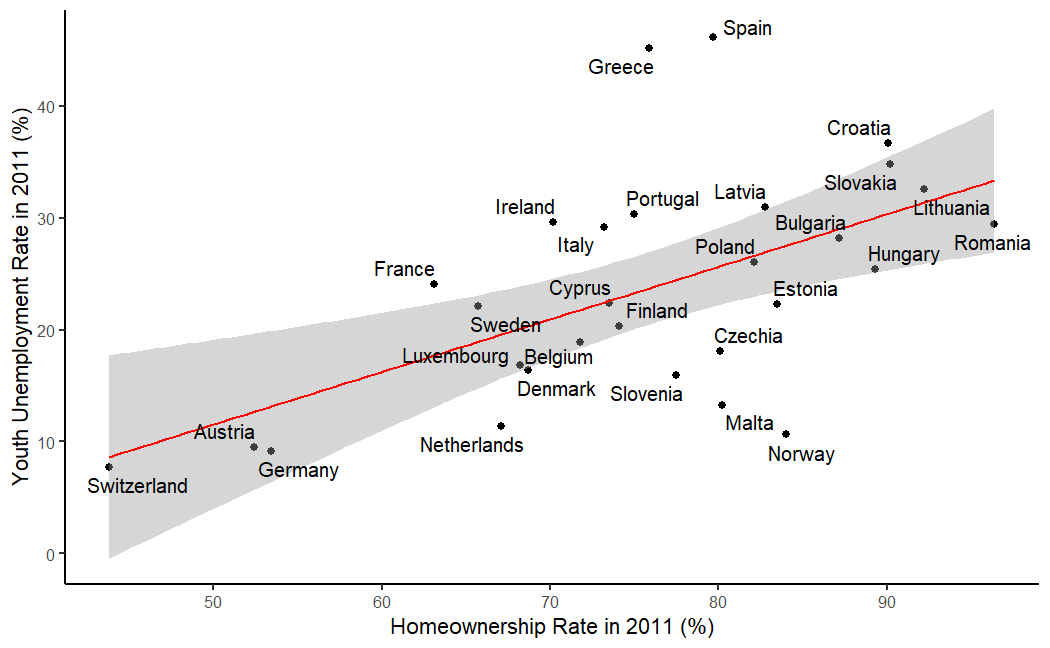
\includegraphics[width=1\linewidth]{youth_unemployment_2011.png}
			\label{fig:youth_unemployment_2011}
		\end{figure}
		
		\vspace{-1em}
		
		\begin{figure}[H]
			\centering
			\caption{Youth Unemployment Trends}
			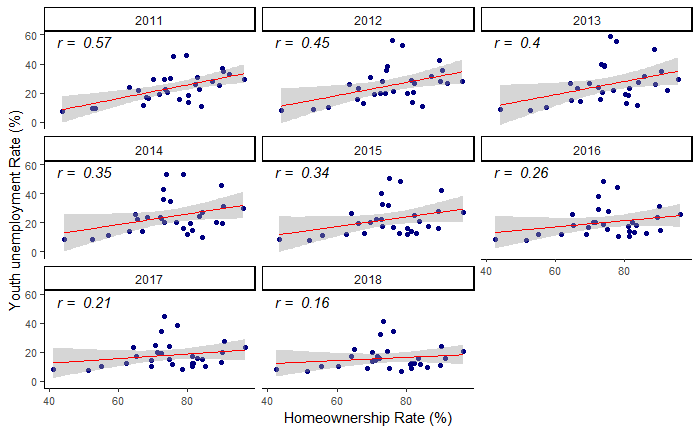
\includegraphics[width=1\linewidth]{youth_unemployment_trends.png}
			\label{fig:youth_unemployment_trends}
		\end{figure}

		\vspace{-1em}
		
		In 2011, countries with higher homeownership rates tended to have significantly higher youth unemployment, with Spain, Greece, and Croatia driving the trend (Figure 1). The correlation was moderately positive and statistically significant (\textit{r = 0.57, p < 0.01}). However, the relationship weakened steadily over time, reaching \textit{r = 0.16} by 2018 and losing statistically significance  (\textit{p = 0.41}). As shown in the faceted plots (Figure~\ref{fig:youth_unemployment_trends}), the initially positive slope flattens over the decade, suggesting a decoupling of homeownership and youth unemployment.
		
		\subsection*{Regression Models}

		\begin{table}[H] \centering 
			\caption{Base Model} 
			\label{} 
			\small
			\begin{tabular}{@{\extracolsep{5pt}}lc} 
				\\[-1.8ex]\hline 
				\hline \\[-1.8ex] 
				& \multicolumn{1}{c}{\textit{Dependent variable:}} \\ 
				\cline{2-2} 
				\\[-1.8ex] & Log Youth Unemployment \\ 
				\hline \\[-1.8ex] 
				Lagged Ownership & 0.018$^{***}$ \\ 
				& (0.003) \\ 
				Constant & 1.602$^{***}$ \\ 
				& (0.212) \\ 
				\hline \\[-1.8ex] 
				Observations & 203 \\ 
				R$^{2}$ & 0.171 \\ 
				Adjusted R$^{2}$ & 0.166 \\ 
				\hline 
				\hline \\[-1.8ex] 
				\textit{Note:}  & \multicolumn{1}{r}{$^{*}$p$<$0.1; $^{**}$p$<$0.05; $^{***}$p$<$0.01} \\ 
			\end{tabular} 
		\end{table} 
		
		\vspace{-1em}
		
		\begin{table}[H] \centering 
			\caption{Added Controls for Year and Country} 
			\label{} 
			\small
			\begin{tabular}{@{\extracolsep{5pt}}lc} 
				\\[-1.8ex]\hline 
				\hline \\[-1.8ex] 
				& \multicolumn{1}{c}{\textit{Dependent variable:}} \\ 
				\cline{2-2} 
				\\[-1.8ex] & Log Youth Unemployment \\ 
				\hline \\[-1.8ex] 
				Lagged Ownership & 0.023$^{**}$ \\ 
				& (0.010) \\ 
				\multicolumn{2}{c}{\textellipsis\ (year and country controls omitted)} \\
				Constant & 1.248$^{**}$ \\ 
				& (0.548) \\ 
				\hline \\[-1.8ex] 
				Observations & 203 \\ 
				R$^{2}$ & 0.942 \\ 
				Adjusted R$^{2}$ & 0.929 \\ 
				\hline 
				\hline \\[-1.8ex] 
				\textit{Note:}  & \multicolumn{1}{r}{$^{*}$p$<$0.1; $^{**}$p$<$0.05; $^{***}$p$<$0.01} \\ 
			\end{tabular} 
		\end{table} 

		\vspace{-1em}

		The regression tables present two fixed-effects models predicting logged youth unemployment. Model 1, which includes only lagged homeownership, shows a significant positive association (\textit{$\beta$ = 0.018, p < 0.01}), indicating that youth unemployment rises by 1.8\% for each 1\% increase in homeownership. Lagged ownership alone explains 17.1\% of the variance (R² = 0.171). Model 2 adds year and country fixed effects, slightly strengthening the effect of lagged homeownership (\textit{$\beta$ = 0.023, p < 0.05}) after accounting for structural and temporal differences. This expanded model now explains most of the variance (R² = 0.942). Demographic controls, such as age structure and education, were tested but excluded due to statistical insignificance and limited explanatory power.

		\vspace{-1em}

		\section*{Policy Implications}
		The findings offer partial support for the Oswald hypothesis that high homeownership can reduce labour mobility and raise youth unemployment. While the observed effect is modest, its persistence after controlling for country and year effects suggests that rigid tenure structures can influence labour market outcomes for young people. The weakening of the relationship after 2015 reflects post-crisis economic recovery, but structural barriers remain in countries with inflexible housing systems, especially in Southern Europe. These results underscore the importance of integrating housing policy into youth employment strategies.
		
		\vspace{-1em}
		
		\section*{Recommendations}
		European policymakers should avoid over-prioritising youth homeownership and instead strengthen access to affordable and flexible rental housing. Targeted investments in transport infrastructure and mobility support can help reduce spatial barriers to employment. Monitoring the relationship between housing tenure and youth unemployment can help identify structural barriers early and guide responsive policy. Ultimately, prioritising youth employment can boost incomes and improve young people's long-term access to housing.
		
		\vspace{-1em}
		
		\section*{Limitations}
		As the analysis is correlational, it cannot establish direct causality between homeownership and youth unemployment. Using one-year lagged effects may overlook longer-term housing impacts, while the lack of subnational data limits the ability to capture within-country variation. The absence of the United Kingdom slightly reduces the representativeness of the sample. The study also does not distinguish between types of homeownership or rental tenure, and the proposed mechanism of reduced mobility is inferred rather than directly tested. Finally, the relatively short timeframe (2011-2018) may not reflect longer-term structural trends or delayed policy effects.

		\vspace{-1em}
		
		\section*{Conclusion}
		This study finds that higher ownership rates are modestly associated with increased youth unemployment in the following year. While the relationship has weakened over time, it remains relevant in countries with inflexible housing markets. As housing and labour markets continue to evolve, European policymakers should remain attentive to how tenure structures affect young people's access to employment opportunities.
		
	\end{multicols}
\end{document}